\chapter{Práctica: Navegación global de un TeleTaxi con GPP}\label{cap.gpp}
 Una vez explicado el contexto, los objetivos y las herramientas empleadas en este proyecto, en este capítulo se detallarán las mejoras de infraestructura y componente académico en la práctica de JdeRobot-Academy denominada ``\textit{TeleTaxi}'', así como el evaluador automático creado y la nueva solución de referencia realizada. Esta práctica ya formaba parte del entorno JdeRobot-Academy, pero se han realizado diferentes mejoras que se describirán a lo largo del capítulo.

\section{Enunciado} \label{sec.enunciado}
El propósito de esta práctica es que un taxi autónomo sea capaz de navegar desde un punto de la ciudad a cualquier otro punto donde tiene que recoger o soltar a un cliente. El usuario humano podrá especificar un punto de destino al robot (taxi) picando con el ratón en algún lugar de la ciudad, cuyo mapa también se muestra en el interfaz gráfico del componente académico. El taxi dispondrá de un mapa de la ciudad y un sensor \textit{\acrfull{gps}} que le proporciona una estimación de su posición en la ciudad. Este vehículo posee un actuador de movimiento basado en velocidad lineal y velocidad de giro.\\ 

El alumno deberá programar el algoritmo de navegación global \acrfull{gpp} para obtener una planificación de la ruta que ha de seguir desde la posición actual del robot hasta la posición destino definida por el usuario en la interfaz gráfica (\acrshort{gui}). Una vez calculada la ruta más corta entre los puntos mencionados, en el \acrshort{gui} se podrá visualizar la ruta en el mapa 2D, así como una imagen con el campo de gradiente calculado por el código del alumno (nos dará información acerca de la ruta en función de la distancia). Una vez calculada la ruta, el alumno deberá proporcionar un algoritmo de pilotaje para que el robot la siga. Este algoritmo deberá tener en cuenta el campo calculado mediante el \acrshort{gpp} y la posición del taxi. 

\section{Infraestructura}
En este punto se comentará el entorno creado para llevar a cabo la práctica. Comenzamos con una descripción del robot que se ha empleado para el desarrollo de la práctica, así como una descripción de los actuadores y sensores que posee este robot, y una explicación de la ciudad por la que se moverá nuestro robot.

\subsection{Coche Taxi\_Holo}
El robot que se ha empleado en esta práctica es un nuevo modelo de robot creado en un programa de modelado 3D (como pueden ser Blender, SketchUp, etc). La versión anterior de ``TeleTaxi'' usaba el modelo \textit{yellowTaxi}, el cual es un robot creado para poder moverse de forma autónoma o teledirigida por un escenario. El nuevo modelo \textit{Taxi\_Holo} posee sensores \acrshort{gps} que le permiten saber cuál es su posición en todo momento; así como motores que le permite moverse por el escenario de manera adecuada. No posee otros sensores como pueden ser cámaras o láseres.\\

El modelo \textit{yellowTaxi} de la versión antigua de la práctica ``TeleTaxi'' es realista, tiene en cuenta las características propias de un automóvil, pero con el aspecto de un taxi. Este robot posee unas dimensiones grandes, ya que mide aproximadamente 5.75 metros de largo, 3 metros de ancho y posee una altura de 3 metros (Figura~\ref{fig.teleTaxi}).  Una característica importante de este modelo es que es  holonómico \footnote{Holonómico quiere decir que puede girar en el sitio sin chocar con nada.}. Este coche  se puede ver en la figura ~\ref{fig.teleTaxi}.

\begin{figure}[H]
  \begin{center}
    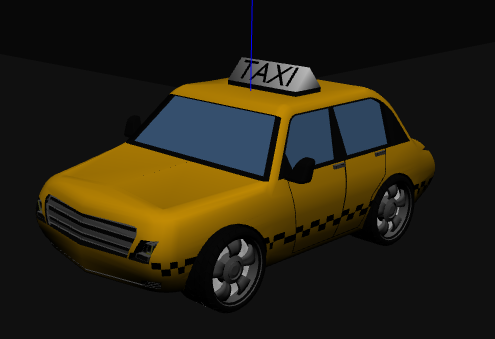
\includegraphics[width=0.3\textwidth]{figures/GPP/gpp_teleTaxi.png}
		\caption{Modelo yellowTaxi}
		\label{fig.teleTaxi}
		\end{center}
\end{figure}

Este modelo tenía fallos en su estructura que hacían que apenas se pudiera desplazar en el mundo o no fuera capaz de rotar, aunque le enviáramos órdenes de velocidad de tracción y velocidad de rotación muy elevadas. Este inconveniente suponía que el taxi tardara mucho tiempo en llegar a un objetivo cercano o que fuera incapaz de girar suficiente en las curvas, lo que hacía que se chocara contra las paredes de los obstáculos. Por este motivo, se creó un nuevo modelo de taxi denominado \textit{taxi\_holo}.\\

El nuevo modelo de taxi (Figura~\ref{fig.coche_holo}), el cual ha sido creado por desarrolladores del proyecto JdeRobot, cuenta con sensores de \acrshort{gps} y motores que permiten el movimiento al igual que el modelo antiguo. Es capaz de moverse de forma fluida por el escenario. Posee unas dimensiones de menor tamaño, 4 metros de largo, 2 metros de ancho y una altura de 1.5 metros. Este taxi pesa 750 kg y es también holonómico como el anterior, pero resuelve de forma eficiente los problemas de movimiento que tenía el antiguo modelo. 

\begin{figure}[H]
  \begin{center}
    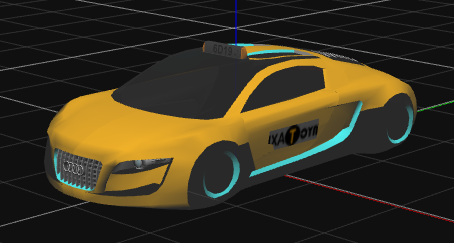
\includegraphics[width=0.3\textwidth]{figures/GPP/Coche_holo.png}
		\caption{Modelo taxi\_holo}
		\label{fig.coche_holo}
		\end{center}
\end{figure}

Los sensores de posición (tipo \acrshort{gps}, odometría u otros) que incorpora el taxi son ampliamente utilizados, ya que son una gran fuente de información para los algoritmos en los que se apoya el pilotaje de nuestro robot. La odometría se emplea para estimar la posición (x, y, orientación) de un robot móvil en todo momento. La posición estimada es relativa a la localización inicial del robot. Por tanto, emplearemos estos sensores de posición para estimar la posición del taxi en el mundo, y a partir de este dato estimar su velocidad.  Los sensores de odometría estiman la posición de las ruedas izquierda y derecha en un intervalo de tiempo determinado. Al conocer las coordenadas de posición anteriores resulta más sencillo obtener la nueva posición de nuestro robot. La plataforma JdeRobot aísla de la complejidad que conllevan los sensores de odometría, facilitándonos una variable que contiene la posición (x, y, orientación) en el mundo.\\


En esta práctica se han empleado dos \textit{plugins} asociados al taxi simulado: 

\begin{itemize}
\item \textit{holoCarPose3d}: Es el \textit{plugin} que emplearán los componentes para poder obtener su posición en tiempo real. También se utiliza para cambiar mágicamente la posición del taxi en el mundo simulado.
\item \textit{holoCarMotors}: Es el \textit{plugin} que permite dotar al taxi de velocidad, tanto velocidad de tracción como velocidad de rotación. 
\end{itemize}

\subsection{Modelo de ciudad cityLarge}
El objetivo de esta práctica es que nuestro taxi sea capaz de navegar por una ciudad hasta un punto destino, por lo que tendremos que crear el entorno (ciudad) donde se moverá. Con este propósito se ha creado un modelo de ciudad llamado \textit{“cityLarge”}. Este modelo fue creado con una herramienta de modelado 3D (Blender). El modelo cityLarge se corresponde con una ciudad de grandes dimensiones. En esta ciudad no veremos casas, semáforos, parques u otros elementos habituales en las ciudades reales, sino que se ha simplificado su creación para que sea rápido en la ejecución del simulador. Mundos con mucho detalle son más costosos computacionalmente de simular. Lo que podremos ver en esta ciudad son bloques que se corresponden con manzanas de edificios o carreteras. También podemos ver elementos propios de las carreteras como son rectas, curvas más simples o curvas pronunciadas, así como una zona amplia que se corresponde con una especie de plaza.  \\

Este modelo se ha modificado respecto a la versión antigua, debido a que en dicha versión debajo de la ciudad había un palo de sujección. Este elemento hacía que el coche adquiriera un poco de movimiento adicional al ejecutar la práctica. Por lo tanto, se ha eliminado este palo de sujeción. \\

En la Figura~\ref{fig.mundo_palo} podemos ver la parte de debajo del modelo \textit{cityLarge} para observar que había un palo de sujeción de la ciudad. En la Figura~\ref{fig.mundo_sinpalo} se observa el nuevo modelo \textit{cityLarge} sin dicho elemento de sujeción. Por último, en la Figura~\ref{fig.citiLarge} tenemos un plano desde arriba de toda la ciudad.

\begin{figure}[H]
  \begin{center}
    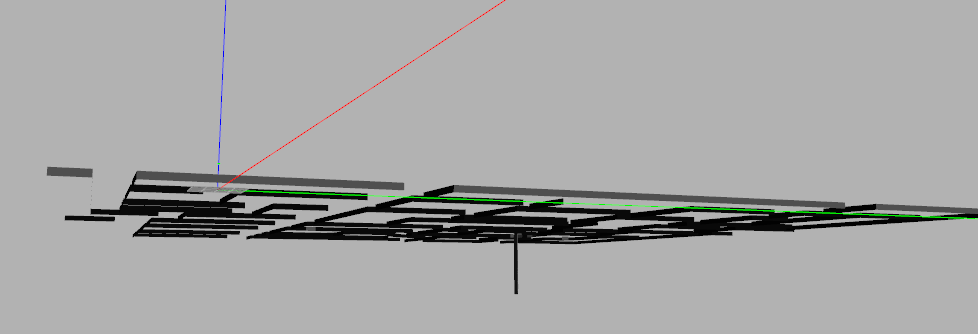
\includegraphics[width=0.6\textwidth]{figures/GPP/Mundo_palo.png}
		\caption{Modelo antiguo cityLarge}
		\label{fig.mundo_palo}
		\end{center}
\end{figure}

\begin{figure}[H]
  \begin{center}
    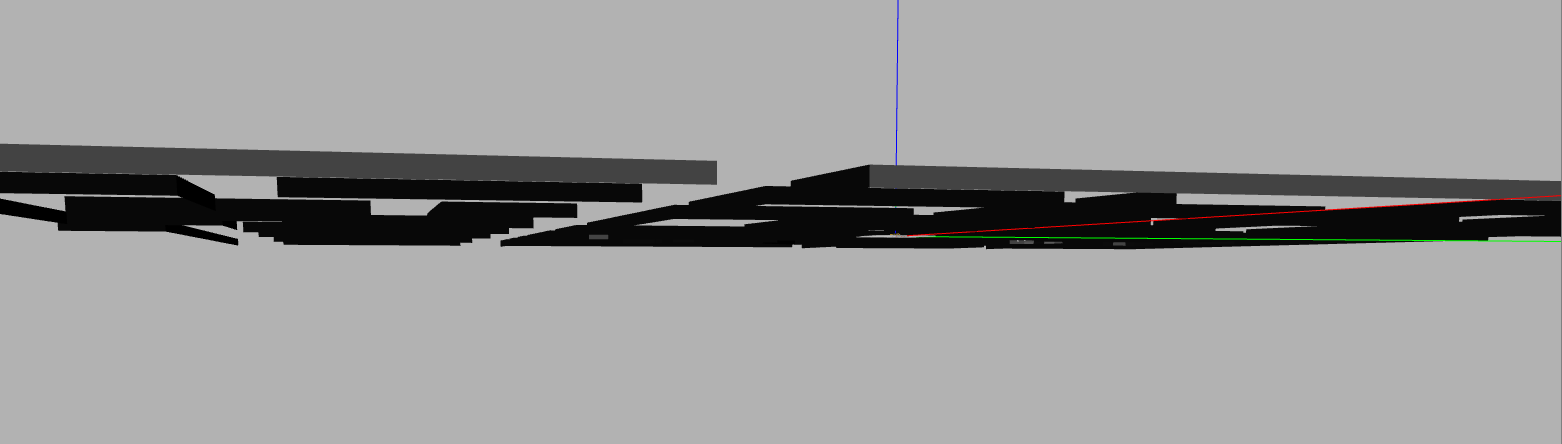
\includegraphics[width=0.6\textwidth]{figures/GPP/Mundo_sinPalo.png}
		\caption{Modelo nuevo cityLarge}
		\label{fig.mundo_sinpalo}
		\end{center}
\end{figure}

\begin{figure}[H]
  \begin{center}
    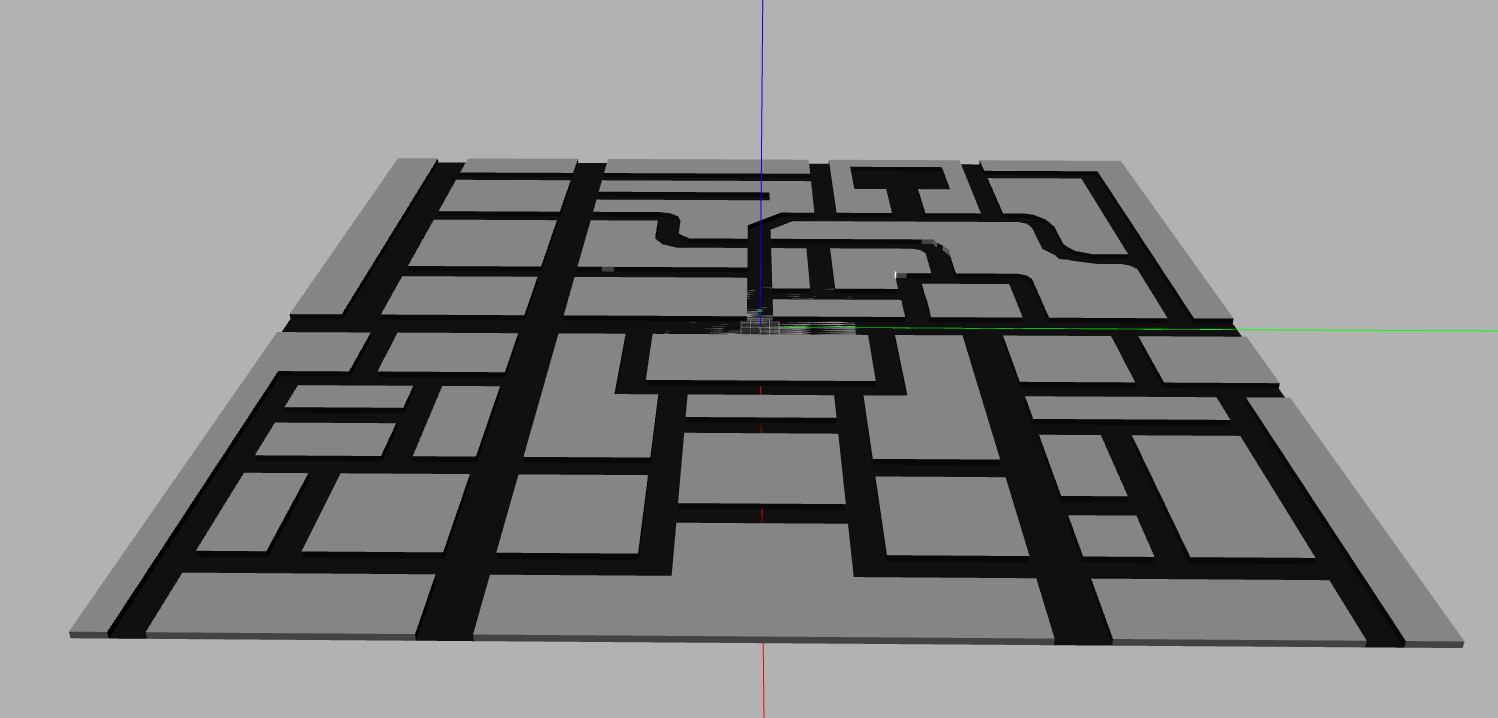
\includegraphics[width=0.5\textwidth]{figures/GPP/citiLarge_modelo.png}
		\caption{Modelo cityLarge desde arriba}
		\label{fig.citiLarge}
		\end{center}
\end{figure}

\subsection{Mundo de Gazebo}
Los mundos que se simulan con Gazebo son mundos 3D. Estos mundos se cargan en ficheros con extensión .world, que no son más que ficheros \acrshort{xml} definidos en el lenguaje \acrshort{sdf}. Este lenguaje contiene una descripción completa de todos los elementos que tiene el mundo y los robots.\\


Se ha creado un mundo en Gazebo (\textit{cityLarge.world}) compuesto por el modelo de la ciudad (\textit{cityLarge}) y el modelo del taxi (\textit{taxi\_holo}). El antiguo mundo en vez de utilizar el modelo \textit{taxi\_holo} empleaba el modelo \textit{yellow\_taxi}. El archivo \textit{cityLarge.world} tiene el siguiente aspecto:

\vspace{20pt}
	\begin{lstlisting}[frame=single]
<?xml version="1.0" ?>
  <sdf version="1.4">
    <world name="cityLarge">
      <!-- My city -->
      <include>
        <uri>model://cityLarge</uri>
      </include>
      <!-- My robots -->
      <include>
        <uri>model://taxi_holo</uri>
        <pose>0 0 0 0 0 0</pose>
      </include>
      <!-- A global light source -->
          <include>
            <uri>model://sun</uri>
      </include>
    </world>
  </sdf>

	\end{lstlisting}

\section{Componente Académico}
El componente académico para ayudar al alumno y alojar su código en esta práctica resuelve varias funcionalidades: (a) ofrece una interfaz gráfica al estudiante que le ayuda a depurar su código; (b) ofrece acceso a sensores y actuadores en forma de métodos simples (oculta el \textit{middleware} de comunicaciones); (c) incluye código auxiliar que no es el foco del algoritmo pero que ayuda a programar la solución. Lo deja todo atado para que el estudiante sólo tenga que incluir su código retocando el fichero \textit{MyAlgorithm.py}.\\

Este componente ofrece al programador del algoritmo un \acrfull{api} de sensores y actuadores. A continuación se puede ver el \acrshort{api} concreto de esta práctica:

\begin{itemize}
\item \textit{sensor.getRobotX()}: Permite obtener la posición del robot en el eje X.
\item \textit{sensor.getRobotY()}: Permite obtener la posición del robot en el eje Y.
\item \textit{sensor.getRobotTheta()}: Permite obtener la orientación del robot con respecto al mapa.
\item \textit{vel.setV()}: Para establecer la velocidad lineal.
\item \textit{vel.setW()}: Para establecer la velocidad de giro.
\end{itemize}

Es necesario escribir un archivo de configuración para que este componente pueda comunicarse con gazeboserver. En este fichero se indican los puertos de los \textit{plugins} que usa el taxi. Este fichero (\textit{teleTaxi.cfg}) en la práctica tiene el siguiente aspecto.

\vspace{20pt}
	\begin{lstlisting}[frame=single]
TeleTaxi.Motors.Proxy = Motors:default -h localhost -p 9999
TeleTaxi.Pose3D.Proxy = Pose3D:default -h localhost -p 9989
TeleTaxi.robot=Pioneer

TeleTaxi.Motors.maxV = 50
TeleTaxi.Motors.maxW = 20

	\end{lstlisting}

Podemos ver que los motores emplean el Puerto 9999, mientras que la pose3d emplea el Puerto 9989. Además, se puede ver en este archivo que se indica al robot la velocidad máxima de tracción y de rotación.\\


Se ha dividido el trabajo de este componente académico en diferentes partes, por lo que emplearemos hilos de ejecución para llevar a cabo diferentes tareas simultáneamente. En esta práctica existen dos procesos diferenciados:

\begin{itemize}
\item Hilo de control: Este hilo es el encargado de actualizar los datos de los sensores y los actuadores a través de las interfaces \acrshort{ice}. El tiempo de refresco de este hilo es muy importante, y debe ser un periodo de tiempo muy corto, ya que se encarga de establecer la velocidad y la dirección del robot en todo momento. Si este tiempo fuera muy grande, las decisiones que modifican la trayectoria del robot podrían ser incorrectas. Este hilo (\textit{ThreadMotors}) se emplea para enviar órdenes a los motores y se actualiza cada 80 milisegundos.

\item	Hilo de la interfaz gráfica de usuario (\acrshort{gui}): Se encarga de ir actualizando la \acrshort{gui}. El intervalo de actualización de este hilo es muy importante. Es necesario que este intervalo sea pequeño, ya que tenemos que mostrar la posición del robot en el mapa en tiempo real. El hilo de ejecución de la \acrshort{gui} (\textit{ThreadGUI}) se actualizará cada 50 ms.

\end{itemize}

\subsection{Interfaz gráfica}

La interfaz gráfica (\acrshort{gui}) de la práctica es una ayuda al alumno para realizar la solución a la práctica. Esta interfaz se realizará en PyQt5, dado que permite realizar interfaces con numerosos objetos gráficos (imágenes, botones, etc).\\


La \acrshort{gui} de la práctica (Figura~\ref{fig.gui_correcta}) contiene una imagen del mapa del mundo de Gazebo a la izquierda. En esta imagen podemos seleccionar el destino al que deseamos que el taxi llegue. En ella se pinta continuamente la posición y orientación actuales del taxi mediante un triángulo azul. El pintado del triángulo se ha modificado puesto que al haber una desviación en la conversión del sistema de referencia del mundo a la imagen o al revés, se había hecho una traslación a la hora de pintar el triángulo que no era necesaria. Esta conversión ha sido eliminada. Además, al cambiar de modelo de taxi se vio que la orientación del taxi no era correcta porque el ángulo no estaba en grados como era de esperar. El ángulo que nos devuelve la orientación del taxi está en radianes. Por lo que se suponía que se debía pasar a grados para poder realizar el pintado del triángulo, pero la conversión era errónea, ya que se multiplicaba simplemente por 100. Esto ha sido modificado obteniendo los grados al multiplicar la orientación por 180 y dividir por \(\pi\). A continuación, podemos ver dos imágenes, una con la orientación del triángulo incorrecta (Figura~\ref{fig.triangulo_girado_mal}) y otra con la orientación correcta (Figura~\ref{fig.triangulo_giro_correcto}).\\

\begin{figure}[H]
  \begin{center}
    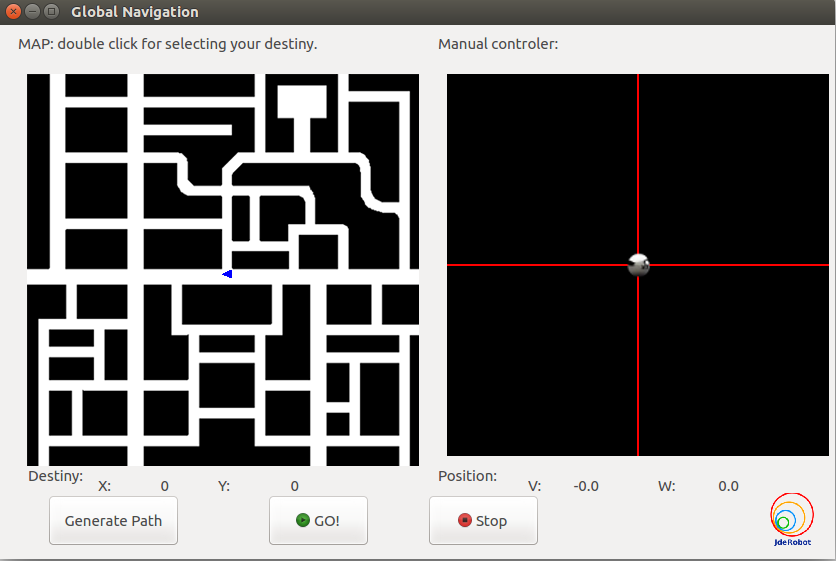
\includegraphics[width=0.5\textwidth]{figures/GPP/GUI_correcta.png}
		\caption{Interfaz gráfica (\acrshort{gui}) actual del \acrshort{gpp}}
		\label{fig.gui_correcta}
		\end{center}
\end{figure}

\begin{figure}[H]
  \begin{center}
    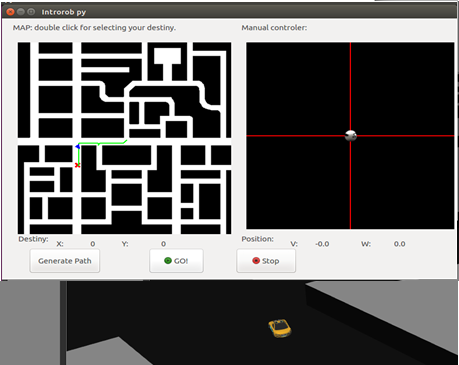
\includegraphics[width=0.5\textwidth]{figures/GPP/triangulo_girado_mal.png}
		\caption{Interfaz gráfica con el triángulo que representa al taxi mal pintado}
		\label{fig.triangulo_girado_mal}
		\end{center}
\end{figure}

\begin{figure}[H]
  \begin{center}
    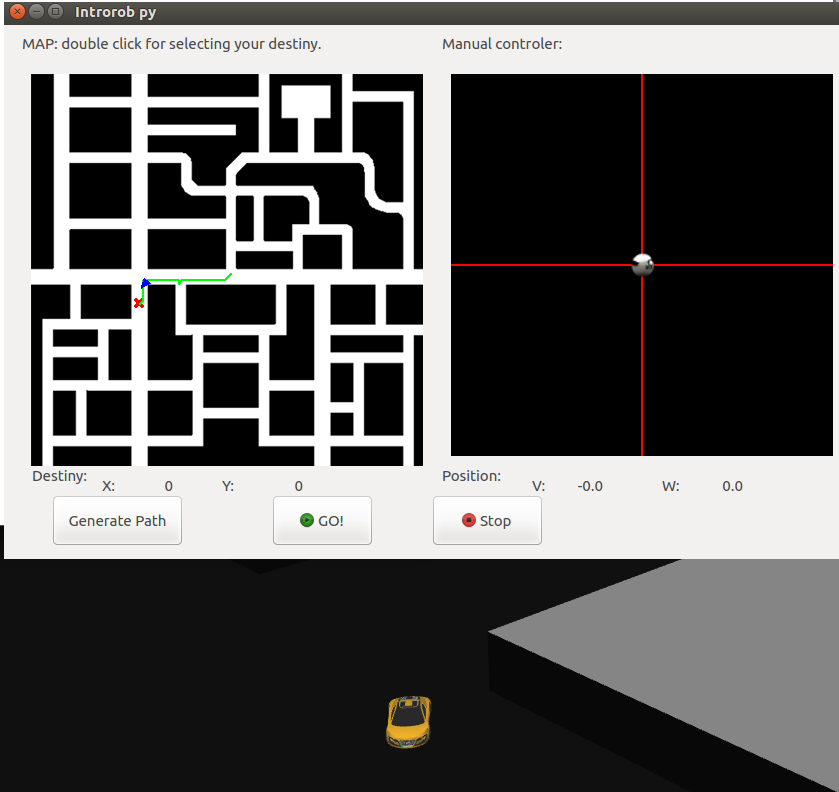
\includegraphics[width=0.5\textwidth]{figures/GPP/triangulo_giro_correcto.png}
		\caption{Interfaz gráfica con el triángulo que representa al taxi correctamente pintado}
		\label{fig.triangulo_giro_correcto}
		\end{center}
\end{figure}

En la interfaz, además se muestra debajo del mapa del mundo la posición numérica exacta que tiene el taxi al iniciarse la práctica en el eje X y en el eje Y. Esta interfaz gráfica (Figura~\ref{fig.gui_correcta}) además muestra un teleoperador a la derecha con el que se puede mover manualmente el taxi en el mundo de Gazebo si se desea.  Por otra parte, debajo del teleoperador podemos ver la velocidad lineal y velocidad angular que tiene al teledirigir el taxi.\\

La \acrshort{gui} posee tres botones, de los cuales dos de ellos serán utilizados para poder ver cómo se lleva a cabo el algoritmo que ha programado el alumno. Cuando pulsamos el botón ``\textit{Generate Path}'', podemos ver el resultado del código que resuelve la parte de la planificación y cómo genera en la imagen del mapa una ruta. De ser pulsado el botón ``\textit{GO!}'' se activará la parte de código que ejecuta el pilotaje del taxi, y podremos ver cómo nuestro taxi navega por las carreteras de la ciudad. El tercer botón sirve para cuando estamos empleando el teleoperador. Este botón nos permitirá parar el taxi si queremos.\\

Se ha modificado el tamaño del visor de la imagen que muestra la \acrshort{gui}, ya que antiguamente no se podía ver la parte inferior del mapa en la \acrshort{gui}, por lo que existían puntos de la carretera a los que no podíamos ir. En las siguientes imágenes se puede comprobar la diferencia que acabamos de mencionar entre la antigua \acrshort{gui} y la actual:
\begin{figure}[H]
  \begin{center}
    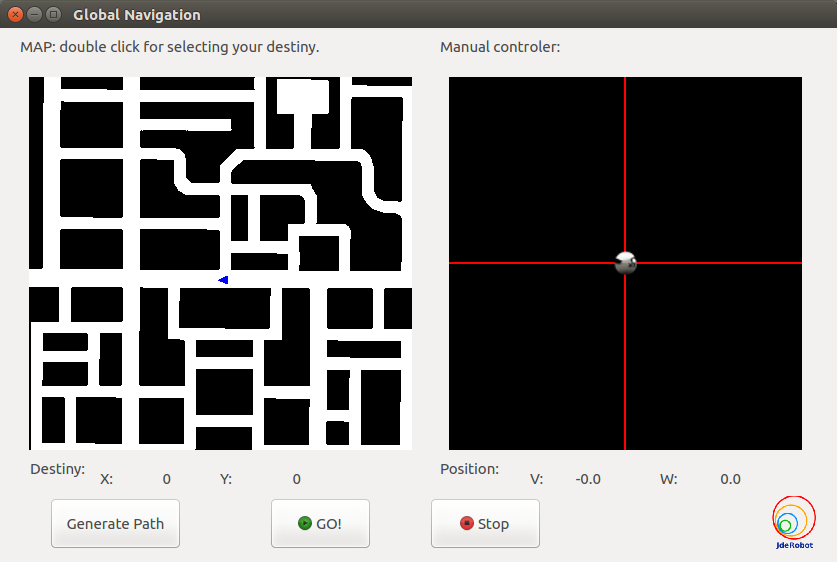
\includegraphics[width=0.5\textwidth]{figures/GPP/GUI_mal.png}
		\caption{Interfaz gráfica (\acrshort{gui}) antigua del \acrshort{gpp}}
		\label{fig.gui_mal}
		\end{center}
\end{figure}

\subsection{Código auxiliar: Clase Grid}
Dentro del componente académico la clase \textit{Grid} se creó en la anterior versión de ``TeleTaxi'', pero se han modificado algunos aspectos en esta versión. Esta clase ofrece un mapa que ayuda al programador a resolver la práctica, permite manipular el mapa de ocupación, crear la rejilla que se emplea para el cálculo del campo y permite controlar la variable ``destino de navegación''.\\

Este componente académico es el que se encarga de capturar información del mundo, crear una rejilla donde se almacenará el campo de la expansión y comunicarse con la interfaz gráfica. Este componente será lanzado al ejecutar la práctica y lanzar la \acrshort{gui}.\\

La clase (\textit{Grid}) será instanciada en el programa principal (\textit{globalNavigation.py}). Cuando es lanzado este componente, se crea una rejilla del tamaño de la imagen del mapa que tiene la interfaz gráfica (400 x 400 píxeles). Esta rejilla se crea para guardar información acerca del mundo. Será utilizada por el alumno para guardar los valores del campo del gradiente (será explicado en el punto~\ref{sec.solucion}) y ayudará a realizar el pilotaje del robot. Además, se inicializa otra rejilla, llamada \textit{path} para almacenar la ruta más corta, la cual se pintará en verde sobre el mapa.\\

Al ejecutar la práctica también se inicializa la variable \textit{map}. Esta variable se inicializa desde la interfaz gráfica y es una imagen binaria del mundo. Tiene representados en negro (valor 0) los píxeles que forman parte de los obstáculos, mientras que los píxeles que forman parte de la carretera serán blancos (valor 255). La imagen será de tres canales, aunque para la solución de la práctica bastará con usar un canal. Este mapa ayudará al alumno a realizar la solución, ya que se puede extraer mucha información de la misma. Esta imagen del mapa ha sido cambiada en la versión actual, debido a que la anterior estaba algo torcida y faltaba una parte del mapa en la parte inferior. Se puede ver en la Figura~\ref{fig.imag_mapa} la diferencia entre la imagen antigua y la actual.

\begin{figure}[H]
  \begin{center}
    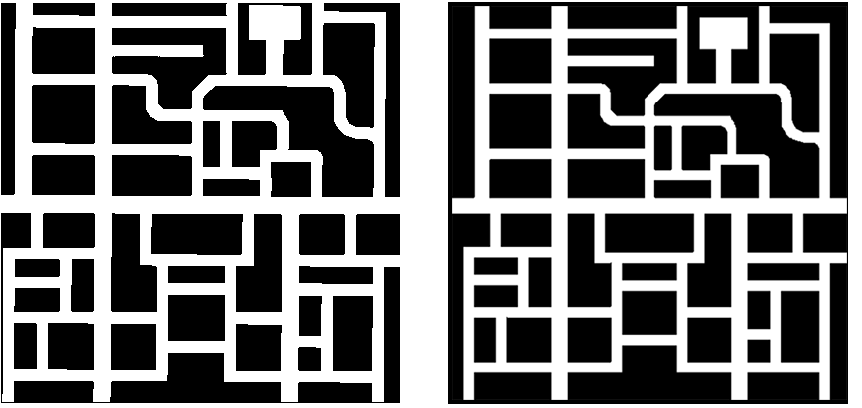
\includegraphics[width=0.8\textwidth]{figures/GPP/imagenes_Mapa.png}
		\caption{Imagen antigua(izquierda) del mapa e imagen actual (derecha)}
		\label{fig.imag_mapa}
		\end{center}
\end{figure}

Este objeto posee una función (llamada \textit{setDestiny}) que será despertada una vez hagamos click sobre la interfaz gráfica para seleccionar el destino deseado. Esta función almacenará las coordenadas del destino en una variable (\textit{destiny}). Esta variable será de gran utilidad para la resolución de la práctica.\\

El objeto \textit{Grid} cuenta con funciones que le permiten relacionarse con el mapa del mundo:

\begin{itemize}
\item \textit{grid.getMap()}: devuelve la imagen del mapa que se está mostrando.
\item \textit{grid.getDestiny()}: devuelve el destino seleccionado en la interfaz gráfica. Este destino se devuelve como una tupla (x, y).
\item	\textit{grid.getPose()}: devuelve la posición respecto al mapa. También será una tupla (x, y).
\item	\textit{grid. showGrid()}: crea una ventana en la que representa los valores del campo que se le han asignado a la rejilla. Los valores más pequeños del campo tendrán un color más cercano a negro, y se irán haciendo más claros a medida que se trate de valores superiores. 
 
\end{itemize}

Este objeto \textit{Grid} también posee funciones que permiten interactuar con la rejilla del campo ficticio (donde se apunta la distancia al destino en ella). Los valores de esta rejilla son de tipo float.  Las funciones son:

\begin{itemize}
\item	\textit{grid.setVal(x, y, val)}: Esta función establece el valor val en la posición indicada (x, y).
\item	\textit{grid.getVal(x, y)}: devuelve el valor de la posición (x, y) del \textit{grid}.
\end{itemize}

El objeto \textit{Grid} consta de funciones que interactúan con la rejilla que contiene la ruta más corta. Los puntos de la rejilla con valor 0 serán ignorados, mientras que los valores superiores a 0 serán considerados parte del camino. Las funciones para interactuar con esta rejilla son:

\begin{itemize}
\item\textit{ grid.setPathVal(x,y, val)}: establece el valor val en la posición indicada (x, y).
\item	\textit{grid.getPathVal(x,y)}: devuelve el valor de la posición indicada (x, y).
\item \textit{grid.setPathFinded()}: indica que se ha encontrado el camino para que empiece a pintarse.
\end{itemize}

Además, esta clase tiene funciones para pasar de coordenadas del mundo a coordenadas del mapa (fila-columna de la rejilla) y viceversa:

\begin{itemize}
\item \textit{gridToWorld(gridX, gridY)}: recibe las coordenadas x e y del mapa \textit{(gridX, gridY)} y devuelve una tupla con las coordenadas equivalentes en el mundo \textit{(worldX, worldY)}.
\item \textit{worldToGrid(worldX, worldY)}: recibe las coordenadas x e y del mundo \textit{(worldX, worldY)} y devuelve una tupla con las coordenadas equivalentes en el mapa \textit{(gridX, gridY)}.

\end{itemize}

Las funciones \textit{gridToWorld} y \textit{worldToGrid} han sido modificadas en la versión actual, puesto que estas funciones tenían un sistema de conversión muy ``ad hoc'' apropiado para cómo estaba hecha la práctica anteriormente, pero no era genérico. Empleaba un sistema de conversión por casos, en vez de emplear matrices de rotación y traslación para pasar de un sistema de referencia a otro. Por eso se ha modificado empleando estas matrices. Uno de los motivos del cambio fue que no era correcta la conversión, sino que era aproximada, lo que provocaba una desviación que afectaba al sistema de pilotaje. Si por ejemplo, teníamos una ruta pintada por el centro de la carretera en la \acrshort{gui}, al realizar el cambio a coordenadas del mundo nos daba como resultado una posición de Gazebo con la cual el coche iba pegado a las paredes, y por ello se chocaba con ellas. En la Figura~\ref{fig.centros} podemos ver la imagen del mapa con la antigua versión (a la izquierda) y la misma con la nueva versión (a la derecha). En este mapa se ha pintado un píxel en rojo en la posición (200, 200), que corresponde con el centro de la imagen, y con la posición donde se encuentra el taxi al lanzar la práctica. 

\begin{figure}[H]
  \begin{center}
    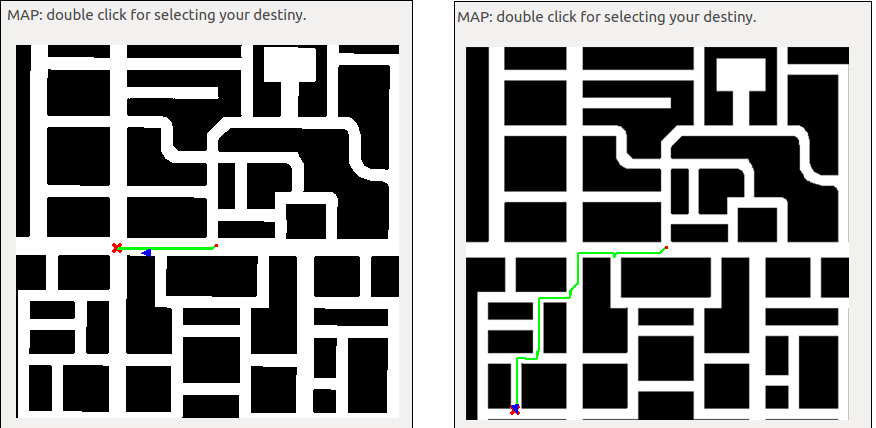
\includegraphics[width=0.8\textwidth]{figures/GPP/centros.png}
		\caption{Imágenes con el centro incorrecto (izquierda) y el centro correcto (derecha)}
		\label{fig.centros}
		\end{center}
\end{figure}

Las matrices de rotación y traslación son muy útiles para pasar de un sistema de referencia del mundo en 3D a un sistema de referencia del mapa en 2D o, al contrario. Estos cambios de sistema de referencia son necesarios porque en la práctica si realizamos la expansión del campo del gradiente sobre una rejilla debemos saber la relación entre cada celdilla de la rejilla con el mundo. Los sistemas de referencia de cada sistema están situados de la siguiente forma:

\begin{figure}[H]
  \begin{center}
    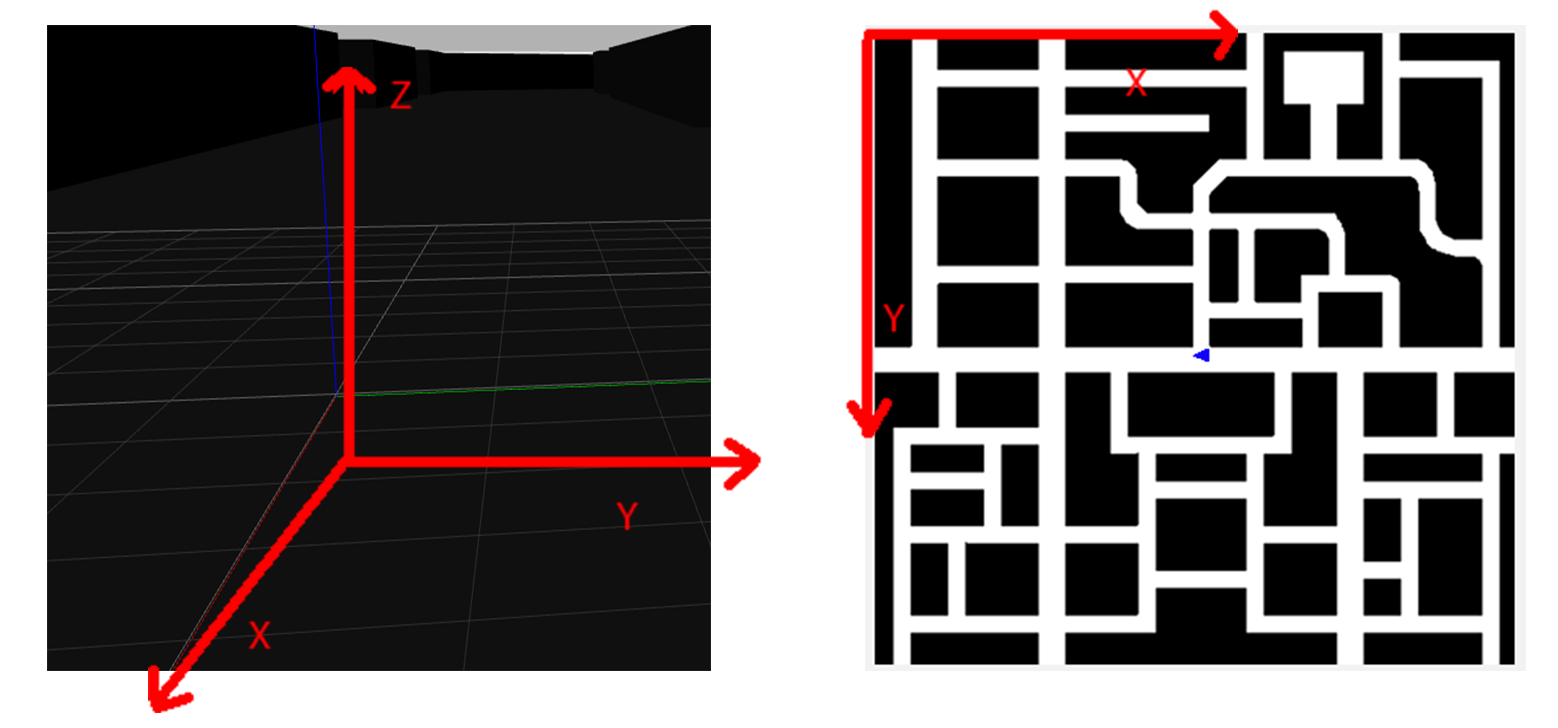
\includegraphics[width=0.8\textwidth]{figures/GPP/referencias.png}
		\caption{Sistema de referencia del mundo (izquierda) y sistema de referencia del mapa (derecha)}
		\label{fig.sistemaref}
		\end{center}
\end{figure}

Para pasar de un sistema a otro deberemos aplicar la rotación y la traslación necesarias. Por ejemplo, en la función \textit{WorldGrid} tenemos que pasar de una coordenada (x, y, z) en un mundo 3D a una coordenada (x’, y’) en 2D. Primero se aplicará una matriz de rotación de \(\pi\) grados sobre el eje x para que el sistema de coordenadas del mundo rote de la siguiente forma:

\begin{figure}[H]
  \begin{center}
    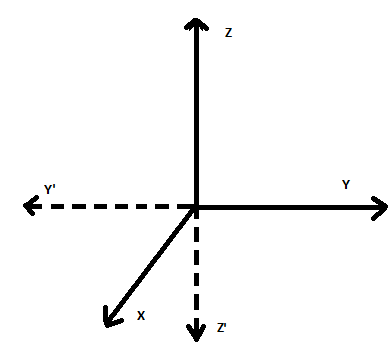
\includegraphics[width=0.4\textwidth]{figures/GPP/Sistema3DRot.png}
		\caption{Rotación sobre el sistema de referencia del mundo (sistema punteado)}
		\label{fig.sistema3DRot}
		\end{center}
\end{figure}

Por si tenemos que aplicar alguna traslación además de la rotación, tenemos una matriz de rotación y traslación para el eje x. Si no queremos realizar una traslación los puntos tx, ty, y tz tendrán valor 0. La traslación se debe a que queremos tener el punto (0,0) de la imagen en la esquina superior izquierda. El cambio lo realizamos siguiendo la ecuación~\ref{ec.matriz}.

\begin{equation}
\label{ec.matriz}
\left[\begin{array}{cc}
x' \\ 
y' \\
z' \\
1
\end{array}\right] = \left[\begin{array}{cccc}
1 & 0 & 0 & tx \\ 
0 & \cos(\alpha) & -\sin(\alpha) & ty\\
0 & \sin(\alpha) & \cos(\alpha) & tz \\
0 & 0 & 0 & 1
\end{array}\right]* \left[\begin{array}{cc}
x \\ 
y \\
z \\
1
\end{array}\right]
\end{equation}
\\

Lo siguiente que tendremos que hacer es aplicar una rotación de –\(\pi\)/2 grados sobre el eje z y una traslación si los puntos están un poco desviados. La traslación será de 200 píxeles (ancho de la imagen/2) en x y -200 píxeles (-alto de la imagen/2) en y. Por lo tanto, tx será en este caso 200, y ty será -200, tz será 0. La matriz de rotación y traslación la aplicamos de la siguiente forma:

\begin{equation}
\left[\begin{array}{cc}
x' \\ 
y' \\
z' \\
1
\end{array}\right] = \left[\begin{array}{cccc}
\cos(\alpha) & -\sin(\alpha) & 0 & tx \\ 
\sin(\alpha) & \cos(\alpha) & 0 & ty\\
0 & 0 & 1 & tz \\
0 & 0 & 0 & 1
\end{array}\right]* \left[\begin{array}{cc}
x \\ 
y \\
z \\
1
\end{array}\right]
\end{equation}
\\

Para realizar la conversión de la imagen al mundo deberemos aplicar las matrices de rotación inversas a estas. 

\section{Solución de referencia}\label{sec.solucion}
El objetivo de esta práctica es proveer al robot de un algoritmo de navegación, que estará compuesto por un algoritmo de navegación global y otro de pilotaje. El algoritmo de cálculo del campo (navegación global) se realizará en una iteración sin tiempo límite, y el algoritmo de pilotaje responde a un control reactivo. En esta sección abordaremos una breve explicación sobre navegación autónoma de robots, una descripción de la técnica \textit{Gradient Path Planning}, y la solución concreta de la práctica. El fichero \textit{MyAlgorithm.py} donde se inserta el código de la solución de referencia es de naturaleza iterativa, ejecuta continuamente iteraciones y en cada una de ellas se percibe y se controla. El alumno tiene que rellenar con su código la función \textit{execute}, que el componente académico invoca periódicamente.

\subsection{Fundamentos de la Navegación global y el algoritmo GPP}
El principal problema de los robots móviles es la navegación autónoma. Es la capacidad que poseen los robots para ir desde un punto del espacio a otro cualquiera evitando chocarse con algún obstáculo, ya sean objetos fijos u objetos móviles inesperados. Esta es una tarea compleja, que provee a los robots de grandes capacidades. La navegación de los robots de forma habitual se divide en dos ramas: la navegación global y la navegación local.\\

La navegación global consiste en calcular o planificar una ruta de forma óptima inicialmente para que el robot la pueda seguir. Para llevar a cabo este proceso el robot debe tener un conocimiento previo del escenario por el cual se debe mover. El robot suele tener previamente esta información mediante un mapa del entorno. De no ser así, el robot adquirirá dicho conocimiento construyendo un mapa del entorno por medio de los sensores que posee. La ruta se construye empleando técnicas de búsqueda o planificación, que requieren un tiempo considerable. Ejemplos de estas técnicas son: grafos de visibilidad y \textit{Gradient Path Planning}.\\

Para solucionar el problema de la navegación global, hemos escogido el algoritmo \textit{Gradient Path Planning} (\acrshort{gpp}), que garantiza una trayectoria mínima entre el punto desde el que partimos hasta el punto de destino. La trayectoria calculada no se basa en la distancia euclídea mínima, sino que se incorporan los obstáculos en el cálculo de la trayectoria.\\

Para desarrollar el algoritmo \textit{Gradient Path Planning} hemos partido del trabajo desarrollado por Kurt Konolige~\cite{gradient}, así como de trabajos previos realizados en la Universidad Rey Juan Carlos~\cite{navegacion_autolocalizacion3}~\cite{navegacion_autolocalizacion4}. Esta técnica obtiene el camino óptimo desde el punto de partida hasta el destino.\\

La técnica \acrshort{gpp} consiste en generar un frente de onda circular que parte desde la posición de destino, y que recorre el espacio libre del mapa hasta llegar a la posición de partida del robot. El punto donde está situado el robot es el comienzo de la ruta que recorrerá el robot. En su propagación, el frente de onda asignará valores de forma creciente a cada punto libre del espacio por el que pase. Antes de comenzar la propagación del frente de onda, todos los puntos libres del espacio tienen valor 0. El frente de onda se puede expandir por todo el espacio, hasta la posición que ocupa el robot o un poco más allá.\\

Adicionalmente los obstáculos generarán su propio frente de onda de penalización, lo que implica que los puntos del espacio que estén próximos a los obstáculos aumentarán su valor por defecto considerablemente. El frente de onda de penalización se propaga de forma inversa al frente de onda anterior. Esto quiere decir que los puntos del espacio más próximos a los obstáculos tendrán un valor mayor a los puntos más alejados. El frente de onda de los obstáculos se expande hasta una distancia determinada, no se expanden por todo el espacio.\\

Sumar la expansión del frente de onda de penalización evita que el robot se acerque a los obstáculos al navegar por el espacio. De no ser así, la ruta más corta estaría pegada a los obstáculos, y de esta forma el robot rozaría con las paredes. Esto hará que el robot tenga mayor seguridad.\\

Una vez se ha generado el campo total, el robot podrá navegar hasta el destino evaluando en cada iteración los puntos de su alrededor. Siempre se dirigirá hacia el punto de menor valor del campo calculado. A medida que avance el robot hacia su destino, el campo calculado tendrá menor valor, pues las zonas más próximas al destino son las que menor valor poseen.  \\

El método \acrshort{gpp} permite generar una ruta ideal desde el punto de partida del robot hasta el destino deseado. Esta ruta se generará siguiendo el gradiente del campo calculado, y será la de menor distancia incorporando los obstáculos. Esta técnica de navegación global asegura que llegaremos al objetivo. Sin embargo, es posible que el robot durante el pilotaje no siga exactamente la ruta calculada, pues puede tener desviaciones debidas a la velocidad y rotación del robot. El pilotaje se llevará a cabo de forma reactiva, mirando en cada momento cuál es la celdilla vecina de menor valor a la que debe dirigirse, y si se encuentra próximo a algún obstáculo.\\

La forma reactiva se basa en el ``ahora'', es decir, en cada instante de tiempo evalúa la situación y actúa. No desarrolla una solución inicial y la sigue, sino que va actuando en función de lo que ocurra en cada momento.

\subsection{Construcción del mapa del gradiente}
La navegación global mediante \textit{Gradient Path Planning} se puede implementar de diversas formas. La solución implementada  se desarrolla en el fichero \textit{``MyAlgorithm.py''}. En este fichero podremos observar que la solución se divide en un método en el que se construye el mapa del gradiente, y otro método que se corresponde con el pilotaje del robot.\\

En el método \textit{``generatePath''} del fichero \textit{``MyAlgorithm.py''} llevaremos a cabo el desarrollo del algoritmo que genera el mapa del campo del gradiente. Esta función se ejecutará solamente cuando pulsemos el botón \textit{``Generate Path''} en la \acrshort{gui} (Figura~\ref{fig.gui_correcta}). El escenario estará representado gráficamente por una rejilla, donde iremos almacenando el campo calculado. Esta rejilla es proporcionada por la clase \textit{Grid}.\\

Lo primero que debemos conocer antes de comenzar a generar el campo y expandirlo por la rejilla es el mapa, la posición inicial del robot y la posición de destino deseado. En la práctica, se dispone de un objeto \textit{grid} que permite obtener el mapa a través de la función \textit{grid.getMap()}. Este mapa proporciona información del escenario mediante sus valores, donde el valor 0 representa a los obstáculos y el valor 255 representa la carretera. El destino podrá conocerse, una vez el usuario haya seleccionado el destino deseado en la \acrshort{gui}, mediante la función \textit{grid.getDestiny()}. Por último, podemos obtener la posición del robot respecto al mapa mediante la función \textit{grid.getPose()}.

\subsubsection{Generación campo ficticio de navegación global}
En la función \textit{``generatePath''} inicialmente tendremos un bucle que realiza la propagación de los frentes de onda. Es decir, no tendremos un único frente de onda, sino que vamos a tener diferentes frentes de onda, los cuales se encuentran en una lista ordenada. \\

El bucle de la propagación de los frentes de onda se ejecutará hasta que se expanda el campo un poco más allá de la posición del taxi. En este caso se expandirá hasta 20 celdillas más allá de la celdilla que ocupa el taxi en la rejilla. Este número podría haber sido mayor o menor, pero en el caso de que fuera mayor la propagación tardaría más tiempo en ejecución. Si el número fuera menor tendríamos menos conocimiento de los alrededores iniciales del robot.\\

El punto de partida del frente de onda inicial es el destino, que es la celdilla de la rejilla que posee la distancia 0. Será nuestro primer nodo que expandirá el frente de onda a sus vecinos. Cada nodo expandirá el valor de la distancia a sus 8 celdillas vecinas. Este valor de distancia asignado a las celdillas vecinas será el valor del nodo (distancia) + 1 o el valor del nodo + 1.4 en las diagonales. Cuando se encuentre un obstáculo, se almacenará la celdilla de dicho obstáculo en un array y no se le asignará ninguna distancia. De esta forma aseguramos tener almacenadas las celdillas que pertenecen al borde de un obstáculo para posteriormente penalizar a las celdillas que se encuentren muy próximas a los obstáculos.\\

Cada nodo va a expandir antes el frente a sus vecinos que se encuentren a una distancia +1, y posteriormente expandirá el frente a sus vecinos que estén en una distancia + 1.4. Por lo que se podría decir que el frente de onda de cada nodo se divide en dos frentes de onda. De esta forma nos aseguramos que el frente de onda sea aproximadamente circular (Figura~\ref{fig.primera_expansion_gpp}).

\begin{figure}[H]
  \begin{center}
    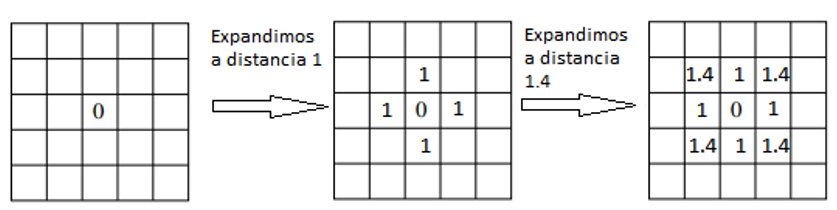
\includegraphics[width=0.8\textwidth]{figures/GPP/primera_expansion.png}
		\caption{Primera propagación del frente de onda}
		\label{fig.primera_expansion_gpp}
		\end{center}
\end{figure}

Este proceso de expansión (Figura~\ref{fig.algoritmo_expansion_gpp}) se irá haciendo sucesivamente hasta llegar a 20 celdillas más alejadas de la posición inicial del taxi. A la hora de realizar la expansión, si las celdillas vecinas tuvieran un valor mayor al que calculara el nodo, dicho valor se actualizaría por el valor que expanda el nodo actual. Esto permite asegurar que siempre tendremos el menor valor posible en cada celdilla.\\

\begin{figure}[H]
  \begin{center}
    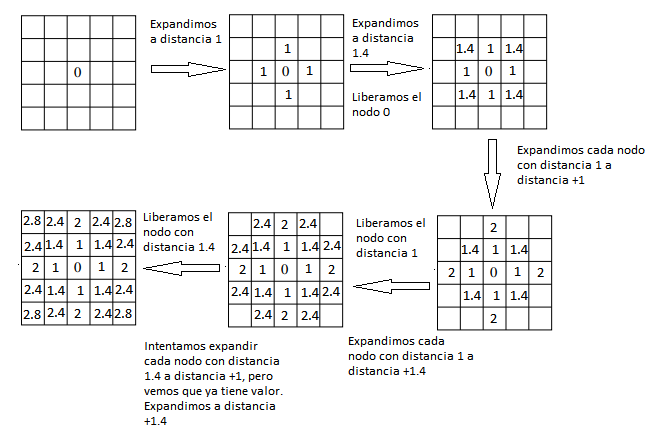
\includegraphics[width=0.8\textwidth]{figures/GPP/algoritmo_expansion.png}
		\caption{Esquema propagación frentes de onda}
		\label{fig.algoritmo_expansion_gpp}
		\end{center}
\end{figure}


En la rejilla del campo que hemos generado (Figura~\ref{fig.expansiones_gpp}) se puede apreciar en color más oscuro los puntos más cercanos al destino, puesto que poseen un valor menor de distancia. Por el contrario, los puntos más lejanos del destino son los que poseerán un color más claro. A continuación, podemos observar una progresión de la expansión del campo.\\

\begin{figure}[H]
  \begin{center}
    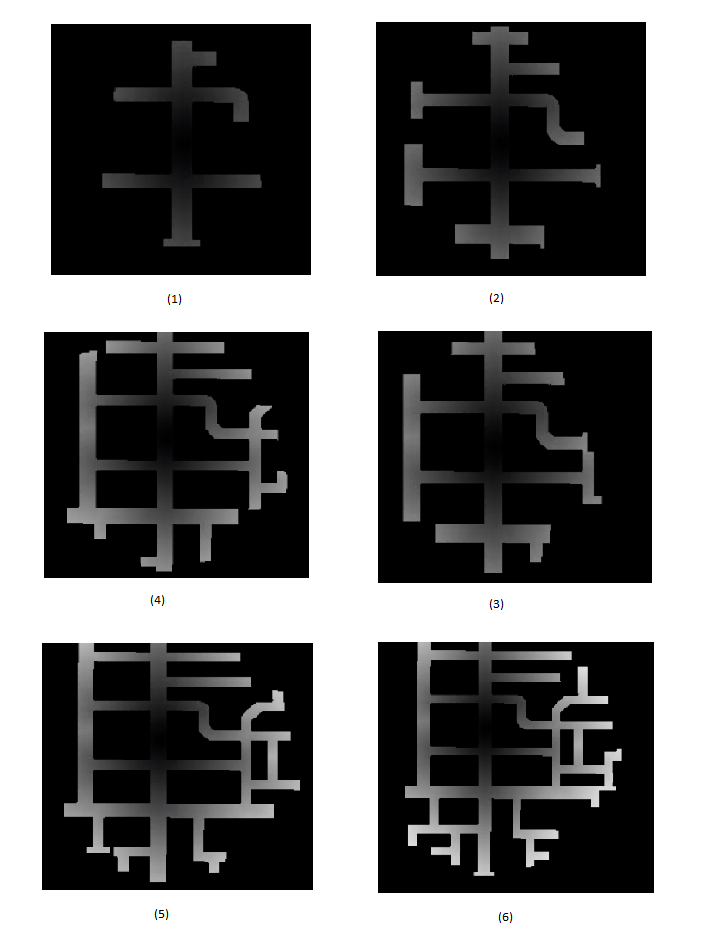
\includegraphics[width=0.8\textwidth]{figures/GPP/expansiones.png}
		\caption{Esquema expansión del campo}
		\label{fig.expansiones_gpp}
		\end{center}
\end{figure}

\subsubsection{Penalización por cercanía de obstáculos}
El segundo paso, es la penalización que realizan los bordes de los obstáculos a las celdillas más próximas. Esta penalización se lleva a cabo para evitar que la ruta más corta desde el robot hasta el destino esté pegada a las paredes de los obstáculos y haga que nuestro taxi roce con las paredes. Con esta penalización nos aseguramos de que en el pilotaje haya un margen de seguridad entre el taxi y las paredes.\\

Como hemos mencionado antes, las celdillas que pertenecen a bordes de obstáculos están almacenadas en un array (llamado \textit{posObstaclesBorder}). Estas celdas (obstáculos) sumarán una penalización a las celdillas vecinas que formen parte de la carretera en función de la distancia a la que se encuentran de la celdilla obstáculo.\\

Para llevar a cabo la penalización por obstáculos se ha creado una nueva rejilla, la cual inicialmente posee un valor 0 en todas sus celdillas. En esta rejilla almacenaremos los valores de penalización. Finalmente sumaremos la rejilla del campo y la de los obstáculos para actualizar sus valores con dichas penalizaciones.\\

La penalización que realizan los obstáculos se llevará a cabo mediante un bucle que recorre el array \textit{posObstaclesBorder}. Cada posición de dicho array penalizará a las celdillas vecinas que están a una distancia de +1, +2 y +3 de la misma. Las celdillas que estén a una distancia de +1 del borde del obstáculo se penalizarán con un valor de 174. Las celdillas con una distancia +2 tendrán una penalización de 168, mientras que las celdillas con una distancia +3 se penalizarán con un valor de 162.\\

En cada penalización que adjuntemos a una celdilla antes comprobaremos su valor en la rejilla de penalización, puesto que dos celdillas del borde del obstáculo pueden querer penalizar a una misma celdilla, pero esta celdilla solamente se puede penalizar una vez. Cuando vayamos a penalizar y comprobemos si ha sido penalizada una celdilla, comprobaremos su valor. Si el valor de penalización que tiene dicha celdilla es menor que el que se iba a añadir, se sustituirá el valor de penalización por el mayor.\\

Estas penalizaciones harán que las celdillas próximas a los obstáculos tengan un valor mayor y aparezcan con un color más claro (blanco) al mostrar el \textit{grid} (Figura~\ref{fig.campos_gpp}). El \textit{grid} lo podemos mostrar mediante la función \textit{grid.showGrid()}. Esta función crea una ventana en la que representa los valores del campo que se le han asignado a la rejilla. Podemos ver en la Figura~\ref{fig.campos_gpp} una serie de ejemplos de diferentes campos calculados con la penalización por obstáculos incluida.\\

\begin{figure}[H]
  \begin{center}
    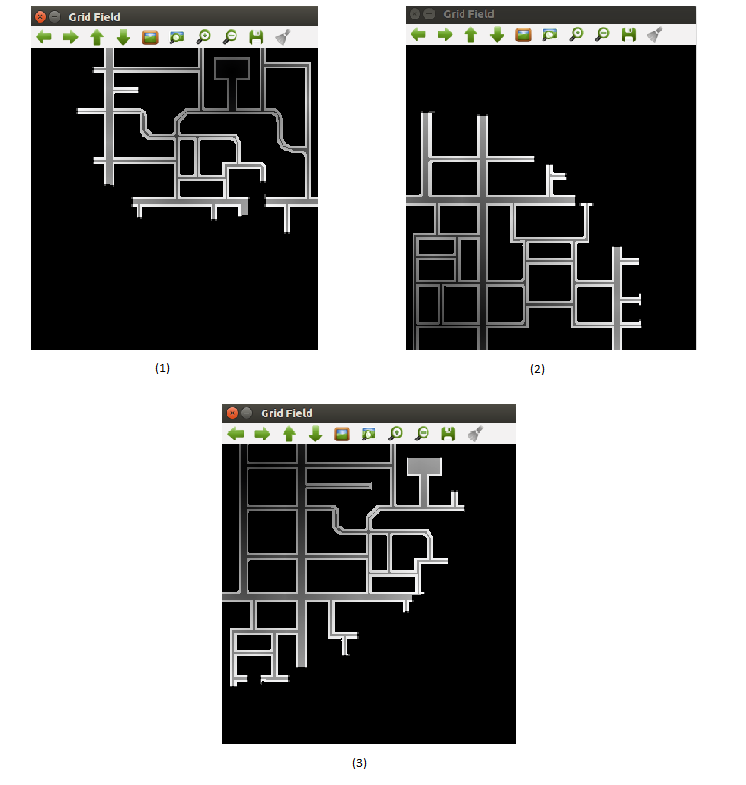
\includegraphics[width=0.8\textwidth]{figures/GPP/campos.png}
		\caption{Representación campos calculados}
		\label{fig.campos_gpp}
		\end{center}
\end{figure}

\subsubsection{Cálculo de ruta ideal}
El paso siguiente es el cálculo de la ruta más corta. Esta ruta se calcula para observar cuál sería la ruta ideal que debe seguir nuestro taxi. Dicha ruta sigue las celdillas de menor valor de distancia.\\


El cálculo de la ruta más corta comienza en la celdilla donde se encuentra situado el taxi y termina al alcanzar la celdilla que posee el valor de distancia 0, es decir, el destino. Para ir almacenando la ruta tenemos que hacer uso de la función \textit{grid.setPathVal}, la cual establece el valor en la posición que se le indica, tomando como ruta las celdillas que poseen un valor diferente a 0. \\

Comenzamos el cálculo de la ruta añadiendo la posición inicial del taxi a la ruta. El siguiente paso es comprobar las celdillas vecinas de la celdilla que ocupa el taxi. Entre estos vecinos añadiremos a la ruta la de menor valor de distancia. Después, comprobaremos los vecinos de esta nueva celdilla y así continuamente hasta llegar a la celdilla destino.\\

Una vez que alcancemos la celdilla del destino tendremos que indicar que hemos terminado de calcular la ruta más corta y que se puede comenzar a pintar. Para ello empleamos la función \textit{grid.setPathFinded}.\\

En la Figura~\ref{fig.rutas_gpp} se pueden observar diferentes rutas calculadas en función del destino que hemos elegido. En las imágenes (1), (2) y (3), podemos ver las rutas calculadas aplicando la penalización de los obstáculos; mientras que en las imágenes (4), (5) y (6) vemos las rutas que se han calculado para los mismos destinos que en (1), (2) y (3), pero sin realizar la penalización de los obstáculos.\\

\begin{figure}[H]
  \begin{center}
    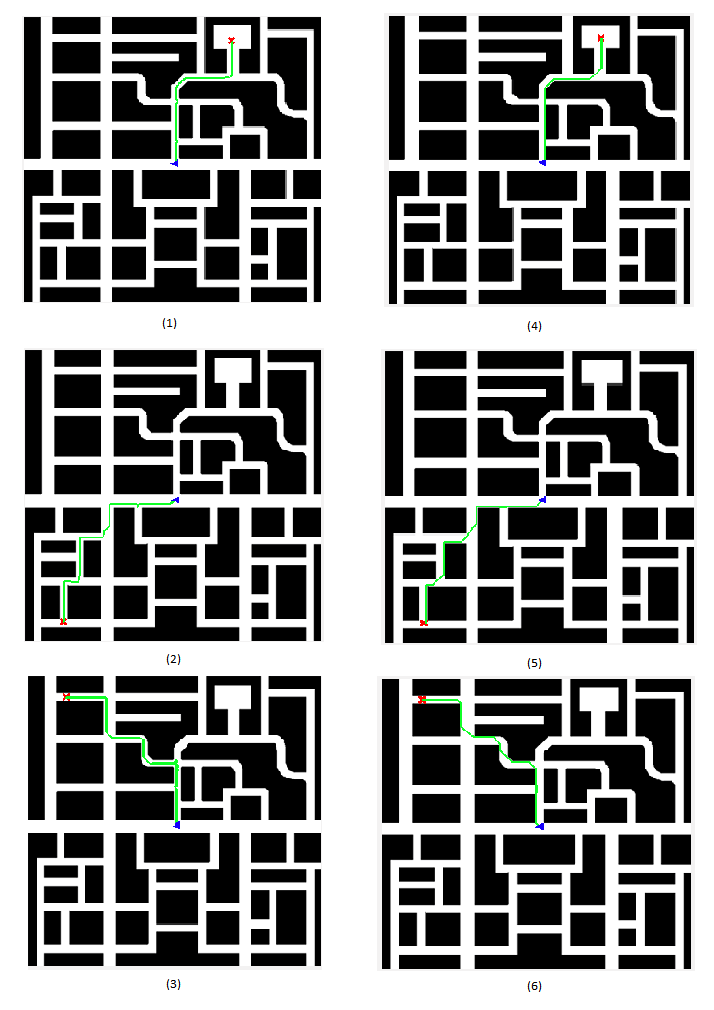
\includegraphics[width=0.8\textwidth]{figures/GPP/rutas.png}
		\caption{Esquema expansión del campo}
		\label{fig.rutas_gpp}
		\end{center}
\end{figure}

\subsection{Pilotaje del robot}\label{sec.pilotaje}
En el método \textit{``execute''} del fichero \textit{``MyAlgorithm.py''} incluimos el código del algoritmo correspondiente al pilotaje del taxi. Este método se ejecuta periódicamente para que el pilotaje sea un control reactivo.\\

Este algoritmo se encarga de pilotar el robot desde su posición inicial hasta la posición del destino mediante el campo calculado en el método \textit{generatePath}. La dificultad está en la elección de la velocidad de tracción y la velocidad de rotación que debemos ordenar al taxi. \\

El pilotaje se ha realizado sin tener en cuenta la ruta más corta calculada en el punto anterior, ya que dicha ruta es el ideal a seguir, pero el taxi al seguir órdenes de velocidad de tracción y de rotación puede desviarse un poco de dicha ruta. Si intentara seguir la ruta ideal estrictamente, el taxi realizaría movimientos muy forzados hasta llegar al destino. Lo ideal es que el taxi se mueva de una forma suave, como lo haría un taxi real. En el pilotaje se ha tenido en cuenta el campo calculado. De esta forma, en cada iteración el taxi irá comprobando el valor de distancia de las celdillas que se encuentran en un cierto radio de distancia con respecto a su posición. De estas celdillas elegirá como objetivo la celdilla de menor valor. Este planteamiento permite que el taxi tenga un comportamiento reactivo ante imprevistos y que se asemeje un poco a la navegación local, ya que no tiene en cuenta únicamente la ruta más corta calculada previamente, también tiene en cuenta la situación del taxi.\\

Inicialmente en el pilotaje debemos comprobar la pose de nuestro taxi mediante el sensor de posición y la posición del destino para ver cuál es la situación del taxi, ya que si el taxi ha alcanzado el destino debe detenerse. Conocemos la celdilla que ocupa el destino en el \textit{grid}, pero el sensor de posición devuelve la posición del taxi con respecto al mundo. Esto implica que debemos convertir las coordenadas del destino en el \textit{grid} en coordenadas respecto al mundo para comprobar si hemos llegado a dicho destino. Para ello se usa la función (\textit{grid.gridToWorld}) que realiza la correspondencia de las coordenadas del \textit{grid} con la posición que tendrían estas coordenadas en el mundo de Gazebo.\\

El siguiente paso es calcular el objetivo local próximo al robot. Vamos a ir calculando en cada iteración un objetivo que se encuentra a cierto radio de distancia del robot. Comprobando los valores de distancia del campo que habíamos calculado en el punto anterior. Por lo que tendremos que obtener la posición del taxi en el sistema de coordenadas del \textit{grid} (mediante la función \textit{worldToGrid}). En nuestro caso comprobaremos las celdillas situadas a una distancia de 5 celdillas con respecto a la posición del robot y escogeremos la de menor valor como objetivo local. El objetivo no es exactamente el anterior mencionado, sino que vamos a calcular un segundo objetivo situado a 5 celdillas del primer objetivo, y posteriormente haremos la interpolación de estos dos objetivos obteniendo el objetivo final al que queremos llegar. El motivo de esta interpolación y ese cálculo doble es obtener un pilotaje con movimientos más suaves. Además, esto nos permite que el taxi gire adecuadamente en las curvas. \\

El objetivo local final calculado está en coordenadas del \textit{grid}, por lo que tendremos que hacer un cambio de coordenadas relativas al mundo para obtener el objetivo en coordenadas del mundo. Una vez lo tengamos, podremos calcular el vector de dirección que tendrá nuestro robot para llegar hasta este y el ángulo. Para ello debemos tener en cuenta la pose que nos devuelve el sensor de posición, así como la orientación del robot (en radianes), las cuales están en coordenadas absolutas del mundo.\\

En esta práctica hay dos sistemas de referencia. Por un lado, tenemos el sistema de referencia absoluto, en el cual se pueden representar la posición del robot y la de cualquier otro objeto. En nuestro caso serán los ejes de Gazebo, por lo cual el punto fijo de referencia será el punto de coordenadas (0, 0, 0) en el mundo de Gazebo. El otro sistema de referencia que vamos a tener en cuenta es el sistema de referencia solidario con el robot. Según se mueva el taxi este sistema de referencia solidario con el robot se desplazará. También hay que mencionar que inicialmente el robot comienza con una rotación de –\(\pi\)/2 radianes.\\

En la Figura~\ref{fig.sistemaReferencia_gpp} podemos ver el sistema de referencia absoluto (son los ejes finos azul, verde y rojo que atraviesan la imagen) y el sistema de referencia solidario con el robot (flechas gruesas azul, roja y verde que salen del robot):

\begin{figure}[H]
  \begin{center}
    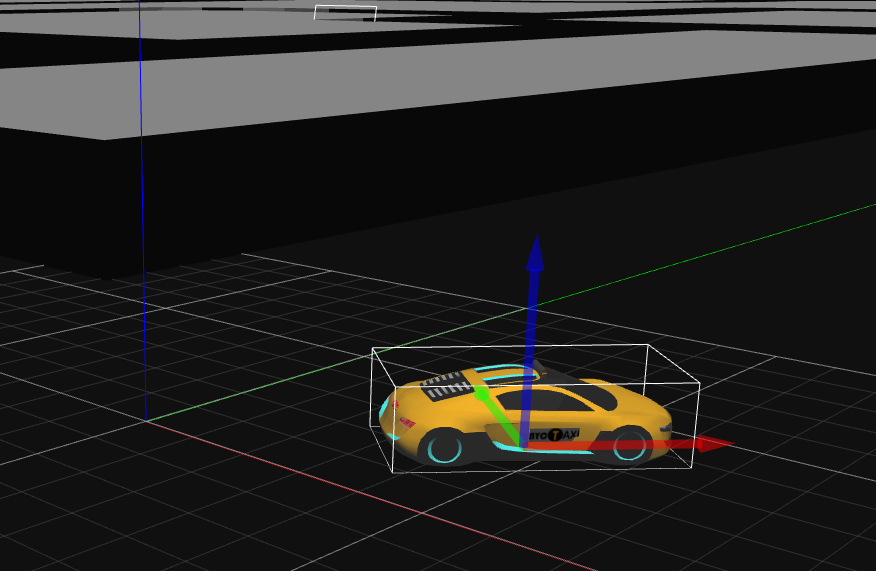
\includegraphics[width=0.5\textwidth]{figures/GPP/sistemaReferencia_GPP.png}
		\caption{Sistema de referencia absoluto (Gazebo) y sistema de referencia solidario con el robot}
		\label{fig.sistemaReferencia_gpp}
		\end{center}
\end{figure}

Se ha decidido definir el sistema de referencia solidario con el robot de la siguiente forma: el eje X de este sistema es el que señala al frente del robot, mientras que el eje Y es el que señala a la izquierda del robot. El origen de este sistema es un punto situado en el centro geométrico del robot.

\begin{figure}[H]
  \begin{center}
    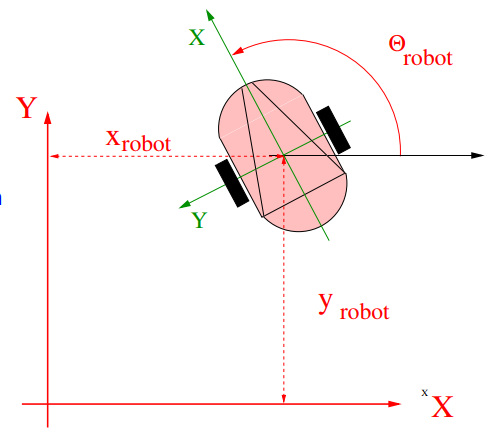
\includegraphics[width=0.5\textwidth]{figures/GPP/sistemasReferencia.png}
		\caption{Sistema de referencia absoluto y sistema de referencia solidario con el robot}
		\label{fig.sistemasReferencia_gpp}
		\end{center}
\end{figure}

El sistema de referencia solidario con el robot se emplea para expresar las coordenadas relativas de los objetivos próximos o de obstáculos respecto al robot. Si tenemos un punto P que no se mueve en el espacio para el sistema de referencia absoluto no habrá movimiento, pero para el sistema de referencia solidario con el robot las coordenadas de este punto P varían.\\

Sabiendo las coordenadas absolutas de un punto, y las coordenadas absolutas del robot y su orientación, podemos pasar las coordenadas absolutas a relativas o al revés. En nuestro caso deberemos pasar las coordenadas absolutas de cada objetivo próximo a coordenadas relativas al sistema del robot para calcular la velocidad de tracción y rotación que debe tener el taxi.\\

Con la transformación de coordenadas absolutas a relativas obtenemos un vector de dirección, con el que podremos calcular el ángulo que hay entre el origen del sistema relativo al robot y la posición relativa del objetivo local. Para obtener el vector de dirección hemos creado una función, en la que primero calcularemos la diferencia entre las coordenadas absolutas del objetivo y las coordenadas absolutas del robot (dx, dy), y después a esta diferencia le aplicamos una matriz de rotación para obtener el vector de dirección. En esta matriz de rotación tendremos en cuenta la orientación  (\(\Theta\)) del robot.

\begin{equation} 
x' = dx \cos(\Theta) - dy \sin(\Theta)
\end{equation}

\begin{equation} 
y' = dx \sin(\Theta) - dy \cos(\Theta)
\end{equation}
\\

Con este vector de dirección conocemos dónde se encuentra situado el punto objetivo con respecto a nuestro origen del sistema del robot, ahora podremos calcular el ángulo que debe rotar el robot para alinearse con este punto. Este ángulo lo calcularemos mediante el cálculo del arco tangente. En la Figura~\ref{fig.Triangulo_gpp} podemos ver un dibujo del ángulo \(\alpha\) que queremos calcular y el punto P (objetivo). Conociendo estos datos podemos calcular \(\alpha\) con la arco tangente.

\begin{figure}[H]
  \begin{center}
    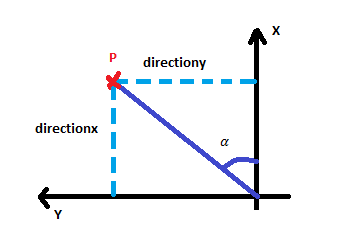
\includegraphics[width=0.5\textwidth]{figures/GPP/Triangulo.png}
		\caption{Sistema de referencia solidario con el robot y punto objetivo}
		\label{fig.Triangulo_gpp}
		\end{center}
\end{figure}

El ángulo \(\alpha\) lo podemos calcular de la siguiente forma:

\begin{equation} 
\alpha = arcotang\left(\frac{directiony}{directionx}\right)
\end{equation}
\\

El ángulo calculado \(\alpha\) está en radianes. Si este ángulo es muy grande significará que debemos dotar al taxi de una velocidad de rotación alta. Por el contrario, si este ángulo es muy pequeño significa que el robot se encuentra más o menos alineado con el objetivo y que probablemente la velocidad de rotación de nuestro vehículo sea 0.\\

En esta solución se ha realizado un control por casos en función del ángulo \(\alpha\)  calculado. En función de este ángulo ordenaremos al taxi mayor o menor velocidad de tracción y de rotación en esa iteración de control. Si el ángulo calculado es muy elevado aplicaremos una velocidad de tracción reducida y una velocidad de rotación elevada (el coche puede estar en una curva o necesitar realizar un gran giro). Sin embargo, si el ángulo es pequeño, le daremos al taxi una velocidad de tracción elevada (ya que se encuentra en una recta) y poca velocidad de rotación.\\

En las Figuras~\ref{fig.camino1_G_gpp},~\ref{fig.camino2_G_gpp},~\ref{fig.camino3_G_gpp} y~\ref{fig.camino4_G_gpp} podemos observar una secuencia de imágenes en la que se ha calculado una ruta y podemos ver cómo aproximadamente el taxi sigue esta ruta, pero a veces se desvía un poco, como habíamos mencionado anteriormente que podría suceder. El taxi alcanza el destino deseado con éxito.

\begin{figure}[H]
  \begin{center}
    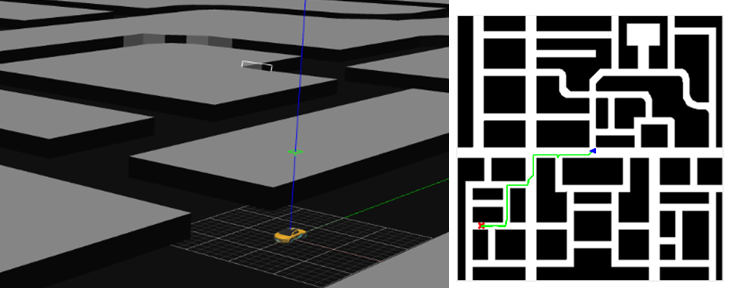
\includegraphics[width=0.8\textwidth]{figures/GPP/camino1_G.png}
		\caption{Posición 1 taxi en el mundo de Gazebo y en la \acrshort{gui}}
		\label{fig.camino1_G_gpp}
		\end{center}
\end{figure}

\begin{figure}[H]
  \begin{center}
    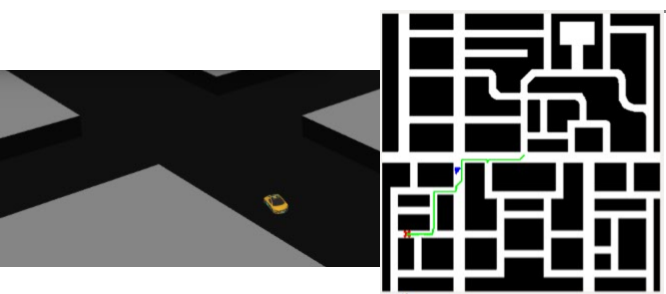
\includegraphics[width=0.8\textwidth]{figures/GPP/camino2_G.png}
		\caption{Posición 2 taxi en el mundo de Gazebo y en la \acrshort{gui}}
		\label{fig.camino2_G_gpp}
		\end{center}
\end{figure}

\begin{figure}[H]
  \begin{center}
    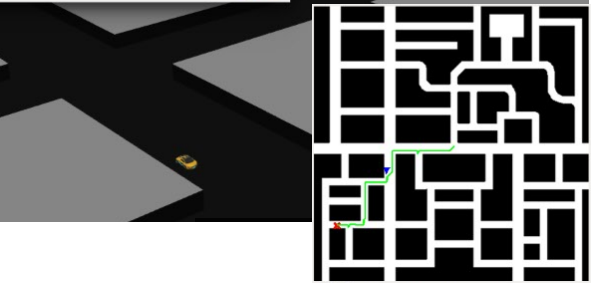
\includegraphics[width=0.8\textwidth]{figures/GPP/camino3_G.png}
		\caption{Posición 3 taxi en el mundo de Gazebo y en la \acrshort{gui}}
		\label{fig.camino3_G_gpp}
		\end{center}
\end{figure}

\begin{figure}[H]
  \begin{center}
    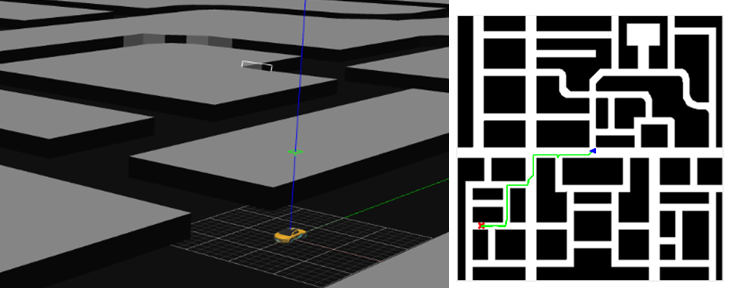
\includegraphics[width=0.8\textwidth]{figures/GPP/camino1_G.png}
		\caption{Posición 4 (destino) taxi en el mundo de Gazebo y en la \acrshort{gui}}
		\label{fig.camino4_G_gpp}
		\end{center}
\end{figure}

\section{Evaluador Automático}
La práctica consta además de un evaluador automático que tiene en cuenta ciertos parámetros para calificar el algoritmo que programa el alumno. Este evaluador automático tiene una interfaz gráfica que muestra los diferentes parámetros, así como la nota final. Para crear el evaluador automático se ha empleado PyQt5 y se han creado clases diferentes para cada parámetro que queramos mostrar. Estas clases serán instanciadas en una clase principal llamada \textit{MainWindowReferee}, que contiene la ventana principal del evaluador automático.\\

\begin{figure}[H]
  \begin{center}
    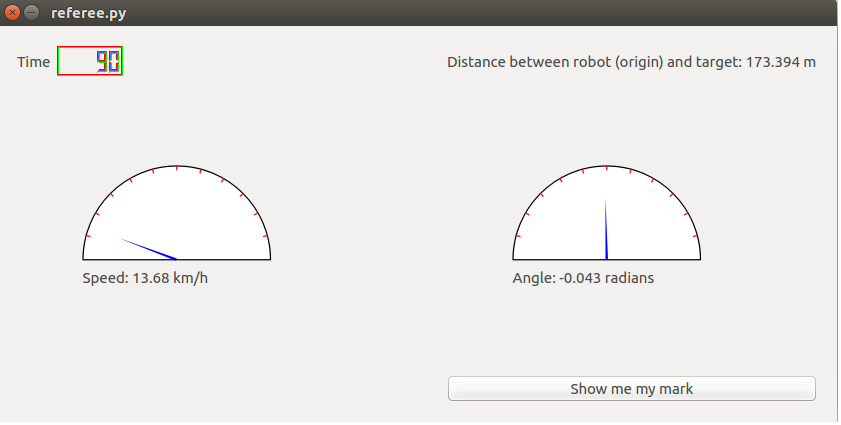
\includegraphics[width=0.7\textwidth]{figures/GPP/referee2_gpp.png}
		\caption{Evaluador Automático del \acrshort{gpp} durante el pilotaje}
		\label{fig.referee2_gpp}
		\end{center}
\end{figure}

El evaluador (Figura~\ref{fig.referee2_gpp}) tiene en su visor un reloj digital que va mostrando los segundos que han pasado desde que se arrancó la práctica. Este visor de tiempo está programado en una clase (llamada \textit{timeWidget}), en la cual se almacenará en una variable los segundos que el taxi está realizando el pilotaje.\\

En segundo lugar, se ha creado una clase (\textit{distanceWidget}) para mostrar la distancia euclídea que existe entre la posición inicial del taxi y el destino que se ha marcado en la \acrshort{gui}. En todos los casos con esta clase se mostrará un mensaje en el visor de la aplicación. Si el destino no ha sido seleccionado todavía mostrará el mensaje \textit{“Distance between robot and target: Destination not yet selected''}. Por el contrario, si ya hemos escogido el destino deseado, mostrará el mensaje: \textit{``Distance between robot (origin) and target: X m”}. Con X nos referimos a que dependiendo de donde esté colocado el destino se mostrará una distancia u otra.\\

En tercer lugar, tenemos un visor de la velocidad (en km/h) que alcanza nuestro taxi durante el pilotaje. En esta clase se realiza un pintado de un velocímetro, que marca con una aguja la velocidad que lleva nuestro vehículo. Cuando el coche está totalmente parado, la aguja aparecerá tumbada hacia la izquierda. Además, debajo del velocímetro aparecerá un mensaje con la velocidad numérica en km/h que tiene nuestro taxi en cada momento.\\

Al igual que sucede con el velocímetro, tenemos un visor similar para pintar la orientación absoluta que tiene nuestro taxi en todo momento, a modo de brújula. Esta orientación irá desde un ángulo de –\(\pi\) (izquierda) a un ángulo de \(\pi\) (derecha). En esta clase (\textit{angleWidget}), también, se mostrará un mensaje con la orientación del taxi.\\

Por último, tenemos la clase que calcula la nota final. En la interfaz gráfica tenemos un botón con el mensaje \textit{``Show me my mark''}. Si pulsamos este botón mostrará nuestra nota. Si el botón se pulsa antes de que el taxi llegue al destino fijado nos indicará en un mensaje que el destino aún no se ha alcanzado. La nota final sólo se calcula si hemos llegado al destino. Si hemos llegado a destino ya tendremos como mínimo una nota de 7, y como máximo una nota de 8, a la cual le sumaremos hasta 2 puntos como máximo en función de la velocidad media del taxi en el pilotaje. Si nos hemos quedado a una distancia máxima de 2 metros del destino tendremos un 8 de nota, a la que le sumaremos hasta 2 puntos como máximo. Por el contrario, si nos quedamos hasta 4 metros de distancia del objetivo el valor de la nota de la que partimos será 7.5; y si por el contrario nos hemos quedado hasta 5 metros del destino, la nota de partida será de 7 puntos. Si nos hemos quedado a más de 5 metros del destino se considerará que no hemos llegado aún. El cálculo del campo del gradiente no se tiene en cuenta en la nota, puesto que es muy difícil comprobar si se ha realizado el cálculo del campo correctamente, ya que hay diferentes modos de realizarlo. Para saber si el campo está bien habría que comprobar la imagen que tenemos como resultado del campo o emplear un vídeo de cómo se realiza la expansión.


\section{Experimentación}

\subsection{Ejecución típica}
Para lanzar la práctica hay que abrir tres terminales y ejecutar en cada uno de ellos:

\begin{enumerate}[1.]
    \item Lanzar Gazebo: gazebo cityLarge.world
\end{enumerate}
\begin{enumerate}[1b.]
\item Si el ordenador que se emplea no tiene muchos recursos se puede arrancar el simulador sin interfaz gráfico: gzserver cityLarge.world
\end{enumerate}
\begin{enumerate}[2.]
    \item Ejecutar el componente académico: python2 globalNavigation.py -- --mapConfig=taxiMap.conf -- --Ice.Config=teleTaxi.cfg
\end{enumerate}
\begin{enumerate}[3.]
  	\item Ejecutar el evaluador automático: python2 referee.py -- --mapConfig=taxiMap.conf -- --Ice.Config=teleTaxi.cfg
 \end{enumerate}

Se han realizado numerosos experimentos con éxito para probar y validar la solución de referencia programada. La ejecución típica representativa ya se ha ilustrado en la Sección~\ref{sec.pilotaje}, que describe una ejecución normal. Una ejecución típica se puede ver en este video \footnote{\url{https://www.youtube.com/watch?v=bNnUfMMXC64}}. 

\subsection{Estudio de tiempos}

En la práctica es muy importante el tiempo de ejecución, ya que este tiempo influye en la nota de la práctica (velocidad media del taxi) y cuanto más rápido sea el algoritmo mejor. En el tiempo que tarda nuestro taxi en llegar al destino, durante el pilotaje, influirá el ordenador que empleemos. Este es un inconveniente, ya que quien posea mejor ordenador obtendrá tiempos de ejecución menores que quien posea un ordenador sin tantas capacidades. La ejecución de Gazebo consume muchos recursos del ordenador haciendo que el taxi sea más lento. \\

En la parte inferior de Gazebo se puede ver el \textit{Real Time}, el \textit{Sim. Time} (tiempo simulado) y el \textit{Real Time Factor}, los cuales tienen mucho que ver en el tiempo de ejecución de Gazebo. El parámetro \textit{Real Time} expresa el tiempo real en ejecución. El factor \textit{Sim. Time} expresa el tiempo simulado. Si utilizáramos un ordenador potente entonces el \textit{Sim. Time} debería estar próximo al \textit{Real Time}. Mientras que si usamos un ordenador sin tantas capacidades veremos que el \textit{Sim. Time} es mucho menor que el \textit{Real Time}. Por su parte, el factor \textit{Real Time Factor} es un producto de la tasa de actualización y el tamaño del paso. Si queremos obtener un tiempo de simulación bajo deberá estar alrededor de 1. Si este parámetro es menor que 1 veremos que la ejecución es más lenta, y cuando se aproxima a 0.2 o menos es demasiado lenta.\\

En el caso del ordenador concreto que se ha empleado el \textit{Real Time Factor} es muy bajo en algunas ocasiones durante el pilotaje, lo que hace que el \textit{Real Time} sea mucho mayor que el \textit{Sim. Time}. En este ordenador el \textit{Real Time Factor} normalmente oscila entre 0.1 y 0.75, siendo en grandes ocasiones cercano a 0.1. \\

En el tiempo total de ejecución de la práctica se puede diferenciar el tiempo de planificación y el tiempo de pilotaje. Dependiendo del destino que elijamos ambos tiempos variarán, siendo menor si escogemos un destino cercano. Se han realizado varias pruebas con diferentes destinos para ver la diferencia entre el tiempo de ejecución.

\begin{itemize}
\item Destino lejano. Hemos elegido un destino bastante alejado de la posición inicial del robot, lo cual se puede observar en la Figura~\ref{fig.experimento1}. Al realizar la prueba, el tiempo de planificación es de tan solo 16’’. El tiempo de pilotaje es bastante mayor, alrededor de 2’ 30’’. Para tener conciencia de cómo influye el ordenador en la ejecución de la práctica, se ha comprobado el tiempo \textit{Real Time} y \textit{Sim. Time} (se inicializan nada más ejecutar la práctica, aunque aún no se haya comenzado a ejecutar el algoritmo) cuando el taxi alcanza el objetivo. El resultado obtenido es que el \textit{Real time} es 3’ 26’’; mientras que el parámetro \textit{Sim. Time} adquiere un valor de 1’ 30’’. La diferencia es excesivamente grande, casi de 2 minutos, lo que implica que en un ordenador con las capacidades al máximo el tiempo de ejecución sería relativamente corto.

\begin{figure}[H]
  \begin{center}
    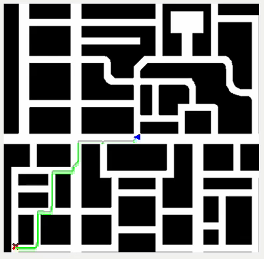
\includegraphics[width=0.4\textwidth]{figures/GPP/Experimento1.png}
		\caption{Imagen del mapa con el primer destino elegido}
		\label{fig.experimento1}
		\end{center}
\end{figure}

\item Segundo destino: En esta ocasión se ha elegido un punto en la plaza, que se podrá ver en la Figura~\ref{fig.experimento2}. Al comprobar el tiempo de planificación se ha obtenido un tiempo de 16’, al igual que en el caso anterior. El tiempo de pilotaje es de 1’ 57’’. En esta ocasión el tiempo de pilotaje ha sido aproximadamente 30’’ más rápido. Si comprobamos el \textit{Real Time} vemos que es de 3’ 06’’; mientras que el \textit{Sim. Time} es de 1’ 35’’. Es decir, en esta ocasión la diferencia entre el tiempo simulado y el tiempo real es menor, lo que nos lleva a obtener un menor tiempo de ejecución.

\begin{figure}[H]
  \begin{center}
    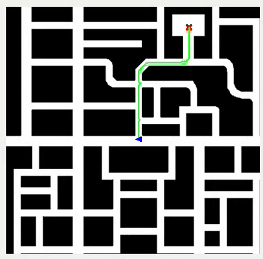
\includegraphics[width=0.4\textwidth]{figures/GPP/Experimento2.png}
		\caption{Imagen del mapa con el segundo destino elegido}
		\label{fig.experimento2}
		\end{center}
\end{figure}

\item Destino a distancia media: El punto escogido lo podemos ver en la Figura~\ref{fig.experimento3}. En este caso el tiempo de la planificación ha sido de 19’, algo superior a las ocasiones anteriores. El tiempo que tarda el taxi en llevar a cabo el pilotaje es de 1’ 12’’, inferior que en el resto de ocasiones puesto que es un destino más cercano. En esta ocasión el \textit{Real Time} ha sido de 2’ 19’’; y el \textit{Sim. Time} ha sido de 1’ 17’’. La diferencia ha sido menor que en las anteriores ocasiones.

\begin{figure}[H]
  \begin{center}
    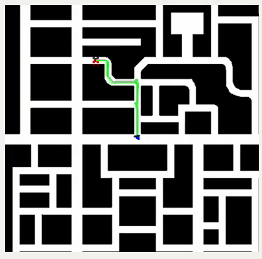
\includegraphics[width=0.4\textwidth]{figures/GPP/Experimento3.png}
		\caption{Imagen del mapa con el segundo destino elegido}
		\label{fig.experimento3}
		\end{center}
\end{figure}
\end{itemize}

Hemos podido comprobar cómo influyen diferentes aspectos en el tiempo de simulación: la lejanía del destino y las capacidades del ordenador que empleemos. Además, hemos observado que el tiempo de planificación suele ser bastante corto, esto es debido a que el algoritmo es rápido. El pilotaje por su parte ha sido más lento debido a distintos aspectos. Sería posible mejorar el tiempo de ejecución empleando quizás algún otro algoritmo más rápido o mejorando el existente. Además, se podría mejorar el tiempo de ejecución dotando al taxi de una mayor velocidad.